\begin{problem}{Photosynthesis}{standard input}{standard output}{1 second}{256 megabytes}

\begin{center}
  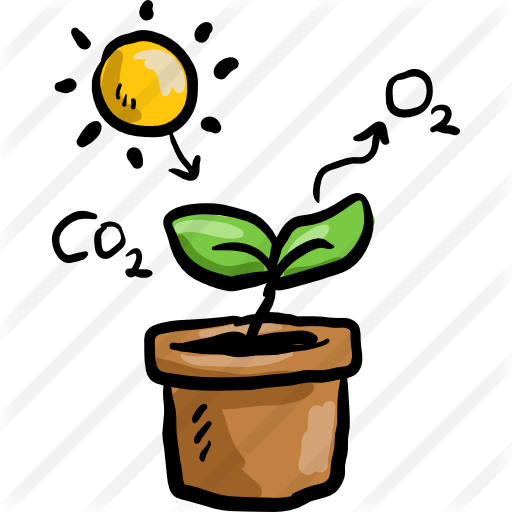
\includegraphics[height=10cm]{photosynthesis-clipart-25.png} \\
\end{center}


Gabriel the Researcher is studying the occurrence of photosynthesis inside the chloroplasts of plants. Photosynthesis is a process used by all plants and some other organisms to convert light energy into chemical energy. Assuming there is unlimited light energy, for every $6$ molecules of carbon dioxide ($\text{CO}_2$) and $6$ molecules of water ($\text{H}_2\text{O}$), $1$ molecule of glucose ($\text{C}_6\text{H}_{12}\text{O}_6$) and $6$ molecules of oxygen ($\text{O}_2$) will be made. Given $a$ molecules of carbon dioxide and $b$ molecules of water, help Gabriel find the number of molecules of glucose and oxygen that will be produced.

\InputFile
The input contains two space separated integers $a$ and $b$ $(0\le a,b\le 10^9)$ "--- the number of molecules of $\text{CO}_2$ and molecules of $\text{H}_2\text{O}$.

\OutputFile
Output two space separated integers "--- the number of molecules of $\text{C}_6\text{H}_{12}\text{O}_6$ and $\text{O}_2$ produced.

\Examples

\begin{example}
\exmpfile{example.01}{example.01.a}%
\exmpfile{example.02}{example.02.a}%
\end{example}

\Note
In the first example, both $14$ molecules of carbon dioxide and $18$ molecules of water allow for $2$ molecules of glucose and $12$ molecules of oxygen. $2$ molecules of carbon dioxide and $6$ molecules of water are left over since they cannot be used in another reaction.


In the second example, since there are $0$ molecules of water, photosynthesis does not take place and no glucose molecules or oxygen molecules are be produced.

\end{problem}

